\documentclass{standalone}
\usepackage{tikz}
\usetikzlibrary{patterns, positioning}


\begin{document}
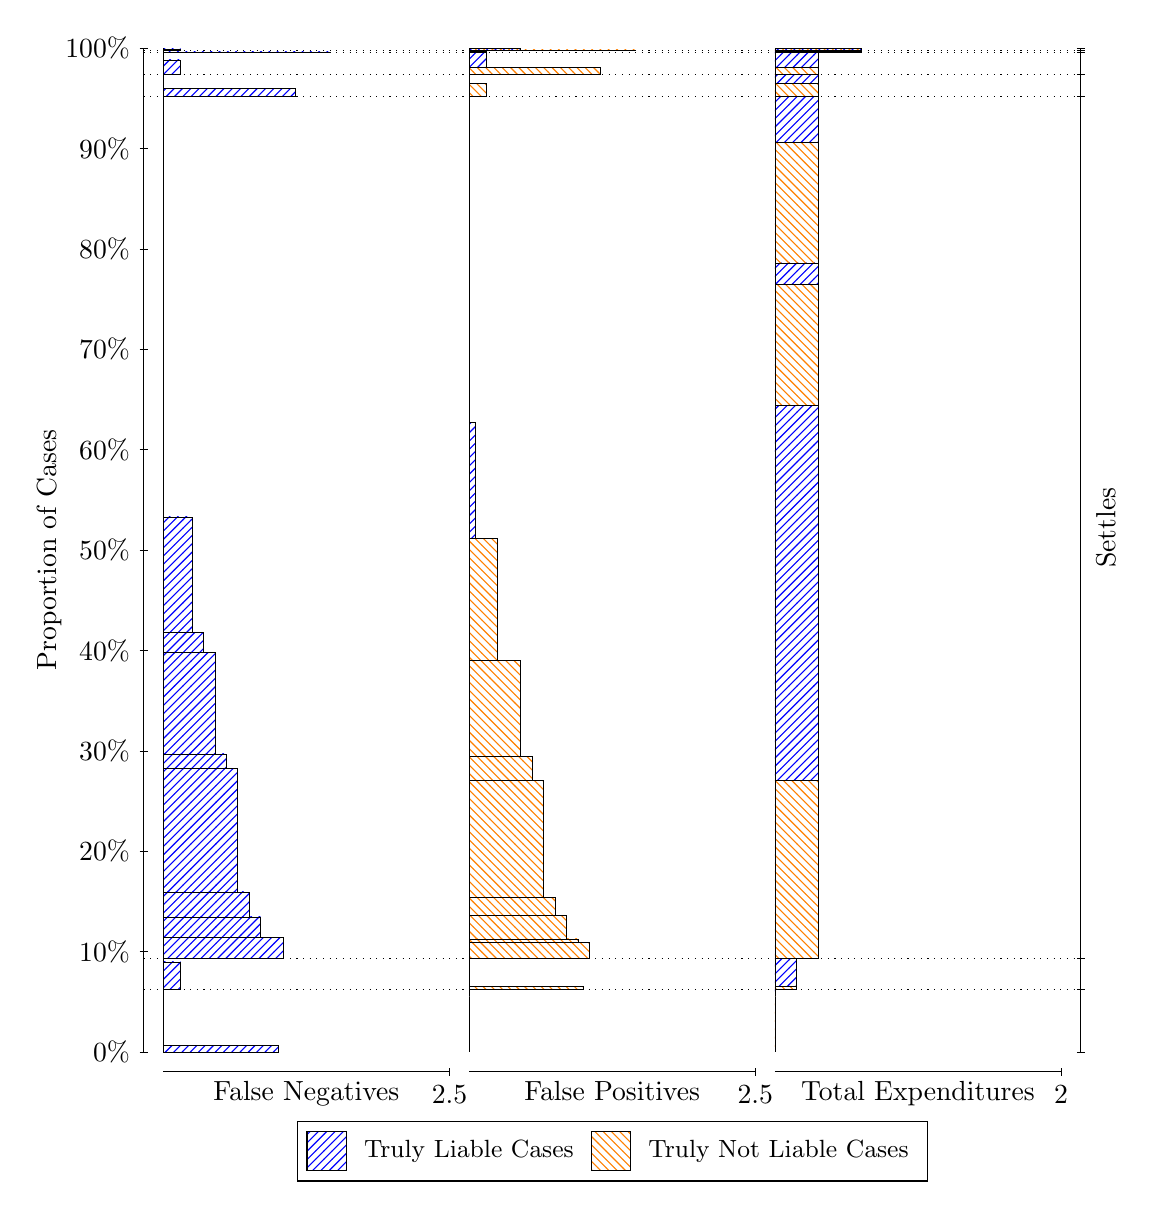
\begin{tikzpicture}
\draw[black, very thin] (1.5,1.75) -- (1.5,14.5);
\node[rotate=90, text=black, anchor=center] at (0.3, 8.125) {Proportion of Cases};
\draw[black, very thin] (1.45,1.75) -- (1.55,1.75);
\node[text=black, anchor=east] at (1.45, 1.75) {0\%};
\draw[black, very thin] (1.45,3.025) -- (1.55,3.025);
\node[text=black, anchor=east] at (1.45, 3.025) {10\%};
\draw[black, very thin] (1.45,4.3) -- (1.55,4.3);
\node[text=black, anchor=east] at (1.45, 4.3) {20\%};
\draw[black, very thin] (1.45,5.575) -- (1.55,5.575);
\node[text=black, anchor=east] at (1.45, 5.575) {30\%};
\draw[black, very thin] (1.45,6.85) -- (1.55,6.85);
\node[text=black, anchor=east] at (1.45, 6.85) {40\%};
\draw[black, very thin] (1.45,8.125) -- (1.55,8.125);
\node[text=black, anchor=east] at (1.45, 8.125) {50\%};
\draw[black, very thin] (1.45,9.4) -- (1.55,9.4);
\node[text=black, anchor=east] at (1.45, 9.4) {60\%};
\draw[black, very thin] (1.45,10.675) -- (1.55,10.675);
\node[text=black, anchor=east] at (1.45, 10.675) {70\%};
\draw[black, very thin] (1.45,11.95) -- (1.55,11.95);
\node[text=black, anchor=east] at (1.45, 11.95) {80\%};
\draw[black, very thin] (1.45,13.225) -- (1.55,13.225);
\node[text=black, anchor=east] at (1.45, 13.225) {90\%};
\draw[black, very thin] (1.45,14.5) -- (1.55,14.5);
\node[text=black, anchor=east] at (1.45, 14.5) {100\%};

\draw[black, very thin] (13.4,1.75) -- (13.4,14.5);
\draw[black, very thin] (13.35,1.75) -- (13.45,1.75);
\node[anchor=west] at (13.35, 1.75) {};
\draw[black, very thin] (13.35,2.5408) -- (13.45,2.5408);
\node[anchor=west] at (13.35, 2.5408) {};
\draw[black, very thin] (13.35,2.9362) -- (13.45,2.9362);
\node[anchor=west] at (13.35, 2.9362) {};
\draw[black, very thin] (13.35,13.881) -- (13.45,13.881);
\node[anchor=west] at (13.35, 13.881) {};
\draw[black, very thin] (13.35,14.162) -- (13.45,14.162);
\node[anchor=west] at (13.35, 14.162) {};
\draw[black, very thin] (13.35,14.441) -- (13.45,14.441);
\node[anchor=west] at (13.35, 14.441) {};
\draw[black, very thin] (13.35,14.467) -- (13.45,14.467);
\node[anchor=west] at (13.35, 14.467) {};
\draw[black, very thin] (13.35,14.5) -- (13.45,14.5);
\node[anchor=west] at (13.35, 14.5) {};

\draw[black, very thin, pattern color=blue, pattern=north east lines] (1.75,1.75) rectangle (3.2033,1.8332);
\draw[black, very thin, pattern color=orange, pattern=north west lines] (1.75,1.8332) rectangle (1.75,2.5408);
\draw[black, very thin, pattern color=blue, pattern=north east lines] (1.75,2.5408) rectangle (1.968,2.8946);
\draw[black, very thin, pattern color=orange, pattern=north west lines] (1.75,2.8946) rectangle (1.75,2.9362);
\draw[black, very thin, pattern color=blue, pattern=north east lines] (1.75,2.9362) rectangle (3.276,3.2015);
\draw[black, very thin, pattern color=blue, pattern=north east lines] (1.75,3.2015) rectangle (2.9853,3.466);
\draw[black, very thin, pattern color=blue, pattern=north east lines] (1.75,3.466) rectangle (2.84,3.7841);
\draw[black, very thin, pattern color=blue, pattern=north east lines] (1.75,3.7841) rectangle (2.6947,5.3538);
\draw[black, very thin, pattern color=blue, pattern=north east lines] (1.75,5.3538) rectangle (2.5493,5.5349);
\draw[black, very thin, pattern color=blue, pattern=north east lines] (1.75,5.5349) rectangle (2.404,6.8233);
\draw[black, very thin, pattern color=blue, pattern=north east lines] (1.75,6.8233) rectangle (2.2587,7.0749);
\draw[black, very thin, pattern color=blue, pattern=north east lines] (1.75,7.0749) rectangle (2.1133,8.5452);
\draw[black, very thin, pattern color=orange, pattern=north west lines] (1.75,8.5452) rectangle (1.75,13.881);
\draw[black, very thin, pattern color=blue, pattern=north east lines] (1.75,13.881) rectangle (3.4213,13.991);
\draw[black, very thin, pattern color=orange, pattern=north west lines] (1.75,13.991) rectangle (1.75,14.162);
\draw[black, very thin, pattern color=blue, pattern=north east lines] (1.75,14.162) rectangle (1.968,14.348);
\draw[black, very thin, pattern color=orange, pattern=north west lines] (1.75,14.348) rectangle (1.75,14.441);
\draw[black, very thin, pattern color=blue, pattern=north east lines] (1.75,14.441) rectangle (3.8573,14.45);
\draw[black, very thin, pattern color=orange, pattern=north west lines] (1.75,14.45) rectangle (1.75,14.467);
\draw[black, very thin, pattern color=blue, pattern=north east lines] (1.75,14.467) rectangle (1.968,14.49);
\draw[black, very thin, pattern color=orange, pattern=north west lines] (1.75,14.49) rectangle (1.75,14.5);
\draw[black, very thin, pattern color=orange, pattern=north west lines] (5.6333,1.75) rectangle (5.6333,2.4576);
\draw[black, very thin, pattern color=blue, pattern=north east lines] (5.6333,2.4576) rectangle (5.6333,2.5408);
\draw[black, very thin, pattern color=orange, pattern=north west lines] (5.6333,2.5408) rectangle (7.0867,2.5824);
\draw[black, very thin, pattern color=blue, pattern=north east lines] (5.6333,2.5824) rectangle (5.6333,2.9362);
\draw[black, very thin, pattern color=orange, pattern=north west lines] (5.6333,2.9362) rectangle (7.1593,3.1456);
\draw[black, very thin, pattern color=orange, pattern=north west lines] (5.6333,3.1456) rectangle (7.014,3.1854);
\draw[black, very thin, pattern color=orange, pattern=north west lines] (5.6333,3.1854) rectangle (6.8687,3.4807);
\draw[black, very thin, pattern color=orange, pattern=north west lines] (5.6333,3.4807) rectangle (6.7233,3.7105);
\draw[black, very thin, pattern color=orange, pattern=north west lines] (5.6333,3.7105) rectangle (6.578,5.1983);
\draw[black, very thin, pattern color=orange, pattern=north west lines] (5.6333,5.1983) rectangle (6.4327,5.5049);
\draw[black, very thin, pattern color=orange, pattern=north west lines] (5.6333,5.5049) rectangle (6.2873,6.7253);
\draw[black, very thin, pattern color=orange, pattern=north west lines] (5.6333,6.7253) rectangle (5.9967,8.272);
\draw[black, very thin, pattern color=blue, pattern=north east lines] (5.6333,8.272) rectangle (5.706,9.7423);
\draw[black, very thin, pattern color=blue, pattern=north east lines] (5.6333,9.7423) rectangle (5.6333,13.881);
\draw[black, very thin, pattern color=orange, pattern=north west lines] (5.6333,13.881) rectangle (5.8513,14.052);
\draw[black, very thin, pattern color=blue, pattern=north east lines] (5.6333,14.052) rectangle (5.6333,14.162);
\draw[black, very thin, pattern color=orange, pattern=north west lines] (5.6333,14.162) rectangle (7.3047,14.254);
\draw[black, very thin, pattern color=blue, pattern=north east lines] (5.6333,14.254) rectangle (5.8513,14.441);
\draw[black, very thin, pattern color=orange, pattern=north west lines] (5.6333,14.441) rectangle (5.8513,14.458);
\draw[black, very thin, pattern color=blue, pattern=north east lines] (5.6333,14.458) rectangle (5.6333,14.467);
\draw[black, very thin, pattern color=orange, pattern=north west lines] (5.6333,14.467) rectangle (7.7407,14.477);
\draw[black, very thin, pattern color=blue, pattern=north east lines] (5.6333,14.477) rectangle (6.2873,14.5);
\draw[black, very thin, pattern color=orange, pattern=north west lines] (9.5167,1.75) rectangle (9.5167,2.4576);
\draw[black, very thin, pattern color=blue, pattern=north east lines] (9.5167,2.4576) rectangle (9.5167,2.5408);
\draw[black, very thin, pattern color=orange, pattern=north west lines] (9.5167,2.5408) rectangle (9.7892,2.5824);
\draw[black, very thin, pattern color=blue, pattern=north east lines] (9.5167,2.5824) rectangle (9.7892,2.9362);
\draw[black, very thin, pattern color=orange, pattern=north west lines] (9.5167,2.9362) rectangle (10.062,5.1983);
\draw[black, very thin, pattern color=blue, pattern=north east lines] (9.5167,5.1983) rectangle (10.062,9.9594);
\draw[black, very thin, pattern color=orange, pattern=north west lines] (9.5167,9.9594) rectangle (10.062,11.506);
\draw[black, very thin, pattern color=blue, pattern=north east lines] (9.5167,11.506) rectangle (10.062,11.771);
\draw[black, very thin, pattern color=orange, pattern=north west lines] (9.5167,11.771) rectangle (10.062,13.298);
\draw[black, very thin, pattern color=blue, pattern=north east lines] (9.5167,13.298) rectangle (10.062,13.881);
\draw[black, very thin, pattern color=orange, pattern=north west lines] (9.5167,13.881) rectangle (10.062,14.052);
\draw[black, very thin, pattern color=blue, pattern=north east lines] (9.5167,14.052) rectangle (10.062,14.162);
\draw[black, very thin, pattern color=orange, pattern=north west lines] (9.5167,14.162) rectangle (10.062,14.254);
\draw[black, very thin, pattern color=blue, pattern=north east lines] (9.5167,14.254) rectangle (10.062,14.441);
\draw[black, very thin, pattern color=orange, pattern=north west lines] (9.5167,14.441) rectangle (10.607,14.458);
\draw[black, very thin, pattern color=blue, pattern=north east lines] (9.5167,14.458) rectangle (10.607,14.467);
\draw[black, very thin, pattern color=orange, pattern=north west lines] (9.5167,14.467) rectangle (10.607,14.477);
\draw[black, very thin, pattern color=blue, pattern=north east lines] (9.5167,14.477) rectangle (10.607,14.5);
\draw[black, dotted] (1.5,2.5408) -- (13.4,2.5408);
\draw[black, dotted] (1.5,2.9362) -- (13.4,2.9362);
\draw[black, dotted] (1.5,13.881) -- (13.4,13.881);
\draw[black, dotted] (1.5,14.162) -- (13.4,14.162);
\draw[black, dotted] (1.5,14.441) -- (13.4,14.441);
\draw[black, dotted] (1.5,14.467) -- (13.4,14.467);
\draw[black, very thin] (1.75,1.5) -- (5.3833,1.5);
\node[text=black, anchor=north] at (3.5667, 1.5) {False Negatives};
\draw[black, very thin] (5.3833,1.45) -- (5.3833,1.55);
\node[text=black, anchor=north] at (5.3833, 1.45) {2.5};

\draw[black, very thin] (5.6333,1.5) -- (9.2667,1.5);
\node[text=black, anchor=north] at (7.45, 1.5) {False Positives};
\draw[black, very thin] (9.2667,1.45) -- (9.2667,1.55);
\node[text=black, anchor=north] at (9.2667, 1.45) {2.5};

\draw[black, very thin] (9.5167,1.5) -- (13.15,1.5);
\node[text=black, anchor=north] at (11.333, 1.5) {Total Expenditures};
\draw[black, very thin] (13.15,1.45) -- (13.15,1.55);
\node[text=black, anchor=north] at (13.15, 1.45) {2};



\node[text=black, centered, rotate=90] at (13.72, 8.4086) {Settles};





\draw (7.449999999999999,1.5) node[draw=none] (baseCoordinate) {};
\begin{scope}[align=center]
        \matrix[scale=0.5, draw=black, below=0.5cm of baseCoordinate, nodes={draw}, column sep=0.1cm]{
            \node[rectangle, draw, minimum width=0.5cm, minimum height=0.5cm, pattern color=blue, pattern=north east lines] {}; &
            \node[draw=none, font=\small, text=black] (B) {Truly Liable Cases}; &
            \node[rectangle, draw, minimum width=0.5cm, minimum height=0.5cm, pattern color=orange, pattern=north west lines] {}; &
            \node[draw=none, font=\small, text=black] (B) {Truly Not Liable Cases}; \\
            };
\end{scope}

\end{tikzpicture}
\end{document}